\begin{frame}{Timing variation inside the bureau: the adjustable-rate resets}
\centering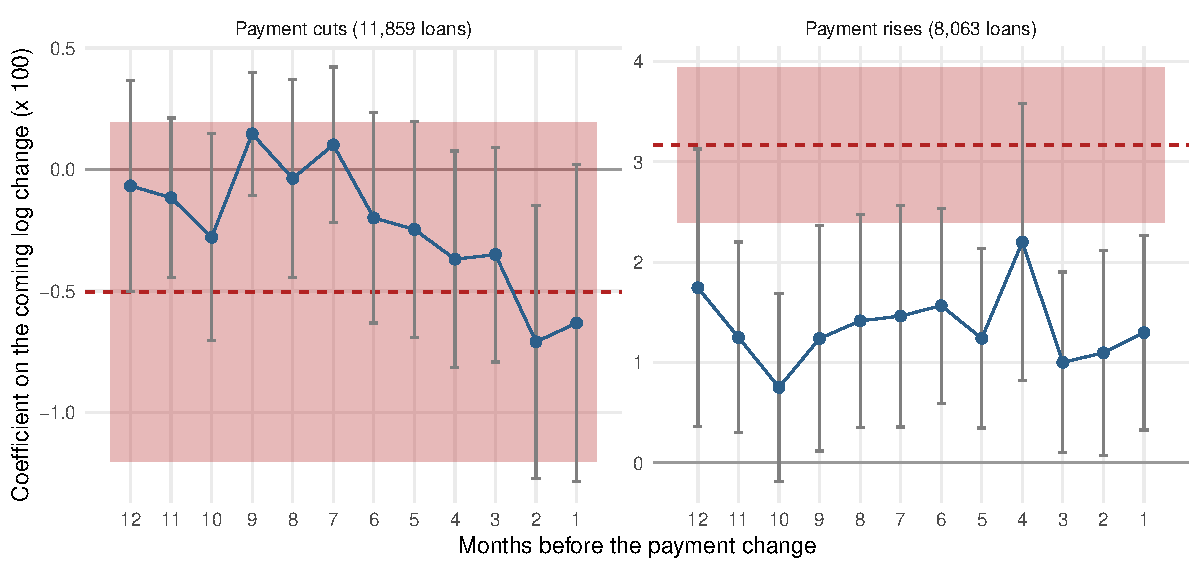
\includegraphics[width=0.9\textwidth,height=0.48\textheight,keepaspectratio]{figures/fig_arm_anticipation.pdf}
\begin{itemize}\small
\m{The panel has no contract flag, so the amortization identity recovers the note rate from the balance path. Of 88,151 payment changes at hybrid reset ages, 9,224 are rate changes, from 6.0 to 3.2 percent at the median.}
\m{At the cut, within loan and vintage month, the response is not distinguishable from zero or from the elasticity of record (1,066 events). Delinquency is higher before a larger coming cut in every sample. Under Proposition 3 the response before a change has the sign of the response at it, so the profile is not a discount function.}
\end{itemize}
\end{frame}
